\documentclass[BCOR10mm]{scrreprt}

\usepackage[utf8]{inputenc}
\usepackage[T1]{fontenc}

\usepackage{lmodern}
\usepackage{graphicx}


\newcommand{\coversheetSubject}[1]{{\large\textbf{\MakeUppercase{#1}}\par}}
\newcommand{\coversheetTitle}[1]{{\Huge\textbf{#1}\par}}
\newcommand{\coversheetAuthor}[1]{{\LARGE#1\par}}


\begin{document}
    \thispagestyle{empty}
    \sffamily
    \parindent0mm

    \vspace*{1.5cm}
    \begin{minipage}[t][9.5cm][t]{\textwidth}
        \begin{center}

            \coversheetSubject{Master's Thesis}

            \par\bigskip\bigskip

            \coversheetTitle{Low Latency Polar FEC Chain \\Development in Software for 5G}

            \par\bigskip\bigskip

            \coversheetAuthor{Yadhunandana R.\ Kumaraiah}

        \end{center}
    \end{minipage}

    \begin{minipage}[t][9cm][t]{\textwidth}
        \begin{center}
            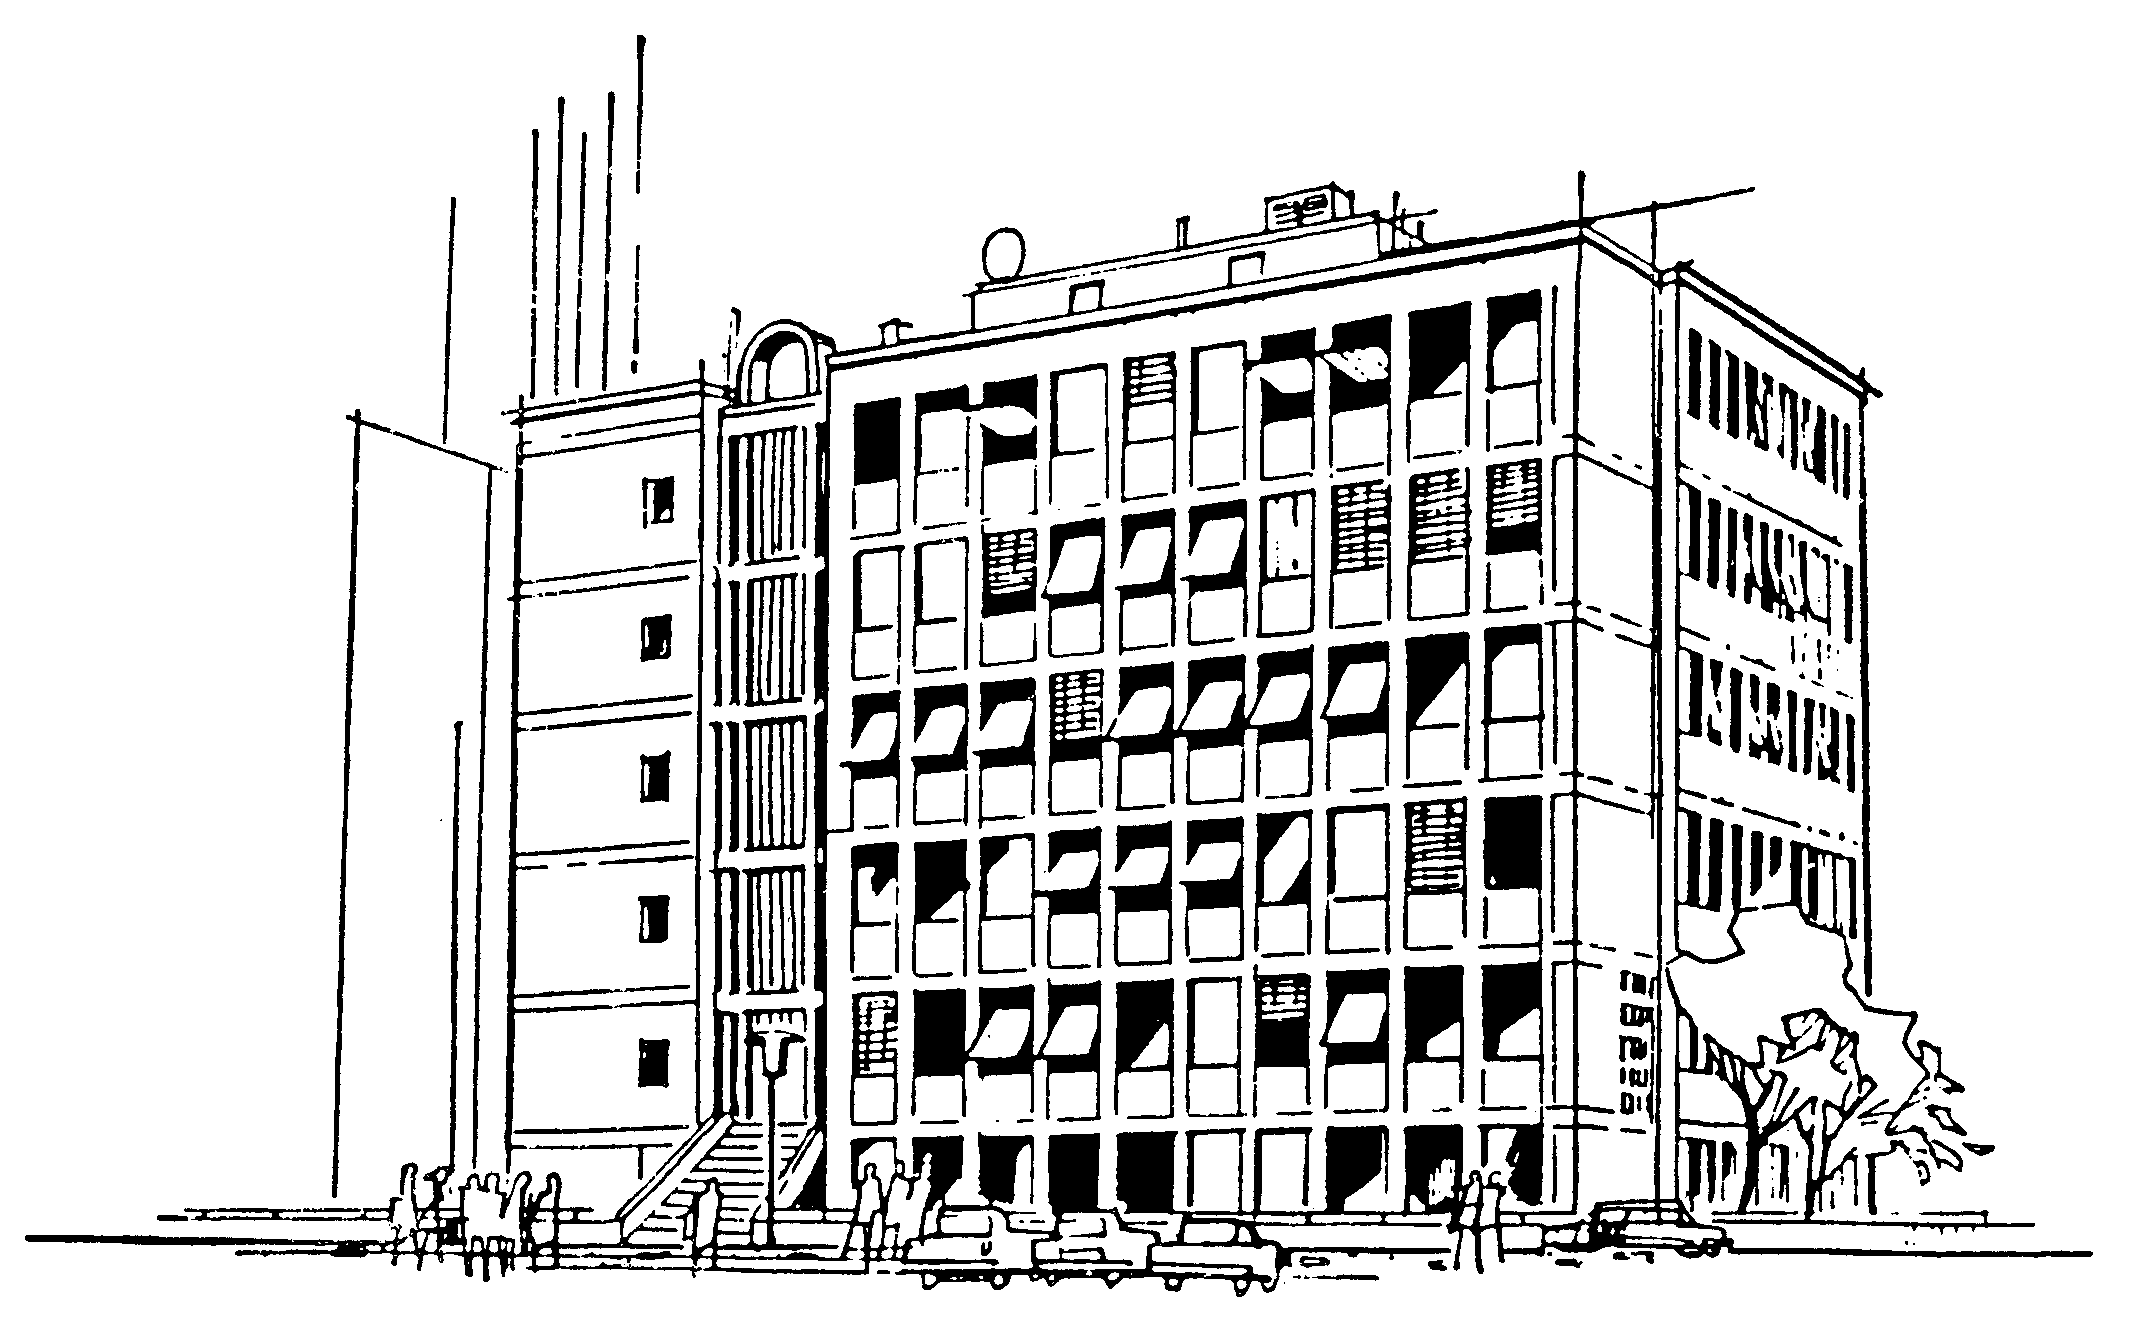
\includegraphics[width=12cm]{figures-template/sketch-n4.png}

            \par\bigskip\bigskip

            {\Large Lehrstuhl für Nachrichtentechnik\\
            Technische Universität München\par}
            {\large Prof.\ Dr.\ sc.\ techn.\ Gerhard Kramer\Large\par}
        \end{center}
    \end{minipage}

\end{document}
